\documentclass[preprint,12pt,aps,pra,showkeys,amsmath,amssymb,superscriptaddress,floatfix]{revtex4-2}
\usepackage[T1]{fontenc}
\usepackage[utf8]{inputenc}
\usepackage{amsmath,amssymb,amsthm,mathtools,mathrsfs}
\usepackage{microtype,booktabs,enumitem}
\usepackage{xcolor,tikz,etoolbox}
\usepackage[skins,breakable]{tcolorbox}
\usepackage{needspace}
% Keep diagram geometry independent of REVTeX preprint body spacing.
\AtBeginEnvironment{tikzpicture}{\linespread{1}\selectfont}
\usetikzlibrary{arrows.meta,positioning,calc,fit,decorations.pathreplacing}
\usepackage{graphicx}
\usepackage{hyperref}

\definecolor{MMBlue}{RGB}{0,82,155}
\definecolor{MMOrange}{RGB}{200,80,0}
\tikzset{
 mmnode/.style={draw=MMBlue,rounded corners=2pt,fill=MMBlue!4,align=left,execute at begin node={\raggedright},text width=5cm,font=\fontsize{10}{12}\selectfont,inner sep=6pt},
 mmimport/.style={mmnode,draw=black!65,fill=black!4},
 mmcandidate/.style={mmnode,draw=MMOrange,dashed,fill=MMOrange!5},
 mmrejected/.style={mmnode,draw=black,densely dotted,fill=black!8},
 mmproof/.style={->,thick,MMBlue},
 mmflow/.style={->,semithick,black!70},
 mmrepair/.style={->,dashed,thick,MMOrange},
 mmcandidatearrow/.style={->,dashed,semithick,MMOrange},
 mmnote/.style={font=\scriptsize,fill=white,inner sep=2pt,align=center}}

\usepackage[section]{placeins}
\setlength{\emergencystretch}{3em}
\setlist{itemsep=3pt,topsep=4pt}
\newtheorem{theorem}{Theorem}[section]
\newtheorem{proposition}[theorem]{Proposition}
\newtheorem{lemma}[theorem]{Lemma}
\newtheorem{corollary}[theorem]{Corollary}
\theoremstyle{definition}
\newtheorem{definition}[theorem]{Definition}
\newtheorem{example}[theorem]{Example}
\theoremstyle{remark}
\newtheorem{remark}[theorem]{Remark}
% Avoid isolated statement headings and single-line paragraph fragments.
\BeforeBeginEnvironment{theorem}{\Needspace{6\baselineskip}}
\BeforeBeginEnvironment{definition}{\Needspace{5\baselineskip}}
\BeforeBeginEnvironment{proposition}{\Needspace{5\baselineskip}}
\BeforeBeginEnvironment{lemma}{\Needspace{5\baselineskip}}
\BeforeBeginEnvironment{corollary}{\Needspace{5\baselineskip}}
\clubpenalty=5000
\widowpenalty=5000
\newcommand{\R}{\mathbb R}\newcommand{\Z}{\mathbb Z}\newcommand{\N}{\mathbb N}
\newcommand{\Pa}{\operatorname{Pa}}\newcommand{\Desc}{\operatorname{Desc}}
\newcommand{\cl}{\operatorname{cl}}\newcommand{\cost}{\operatorname{cost}}
\newcommand{\status}{\operatorname{status}}
% Faculty cards: a visual rail groups the five faculties within one agent.
% The rail has no arrowhead and does not represent a proof dependency.
\newcommand{\mmfacultybadge}[1]{%
 \node[circle,draw=MMBlue,line width=1pt,fill=white,
 minimum size=7mm,inner sep=0pt,font=\sffamily\small\bfseries,text=MMBlue]
 at ([xshift=15pt,yshift=-15pt]frame.north west) {#1};}
\newcommand{\mmfacultyrail}{%
 \draw[MMBlue!80,line width=1pt]
 ([xshift=15pt,yshift=2pt]frame.north west)--
 ([xshift=15pt,yshift=-2pt]frame.south west);}
\newtcolorbox{mmfacultybox}[2]{enhanced,breakable,
 colback=MMBlue!4,colframe=MMBlue!4,boxrule=0pt,arc=3pt,
 left=39pt,right=9pt,top=4pt,bottom=4pt,
 before skip=2pt,after skip=2pt,
 fontupper=\small\linespread{1.1}\selectfont,
 overlay unbroken={\mmfacultyrail\mmfacultybadge{#1}},
 overlay first={\mmfacultyrail\mmfacultybadge{#1}},
 overlay middle={\mmfacultyrail},overlay last={\mmfacultyrail}}
\newcommand{\mmfaculty}[3]{%
 \begin{mmfacultybox}{#1}{#2}
 {\sffamily\bfseries\color{MMBlue}#2}\par\smallskip #3
 \end{mmfacultybox}}
\newcommand{\agent}[9]{%
 \Needspace{8\baselineskip}
 \subsubsection{#1}
 \noindent\textbf{Object.} #2\par
 \noindent\textbf{Role.} #3\par\smallskip
 \mmfaculty{E}{Ego}{#4}
 \mmfaculty{M}{Memory}{#5}
 \mmfaculty{I}{Intellect}{#6}
 \mmfaculty{S}{Sense}{#7}
 \mmfaculty{A}{Action}{#8}
 \smallskip\noindent #9\par}

\usepackage{longtable,array,calc}
\providecommand{\tightlist}{\setlength{\itemsep}{2pt}\setlength{\parskip}{0pt}}
\makeatletter
\def\frontmatter@abstract@produce{\par\addvspace{\frontmatter@preabstractspace}%
\begingroup\prep@absbox\unvbox\absbox\post@absbox\endgroup
\addvspace{\frontmatter@postabstractspace}}
\makeatother
\newcommand{\field}[2]{\par\smallskip\noindent\textbf{#1.} #2\par}
\setlength{\emergencystretch}{5em}
\AtBeginEnvironment{verbatim}{\small\linespread{1.0}\selectfont}


\hypersetup{colorlinks=true,linkcolor=MMBlue,urlcolor=MMBlue,pdfauthor={Dibakar Sigdel}}

\begin{document}

\title{Inverse Function Theorem\\[4pt]\large An End-to-End Meta-Math Walkthrough}

\author{Dibakar Sigdel}

\affiliation{Mindverse Computing LLC, Lynnwood, WA 98087, USA}

\date{October 2026}

\begin{abstract}

A complete authored walkthrough of inverse function theorem, with
explicit mathematical contracts, local verification gates, and reusable
exports. The report presents the target theorem, declared imports, a
dependency graph, five-faculty node contracts, a continuous proof, a
worked example, and a hypothesis-repair audit. It is an authored
mathematical exposition, not a deployed-agent transcript or a formal
proof-assistant certificate.

\end{abstract}\maketitle\linespread{1.12}\selectfont

\noindent\textbf{AC-04 / Advanced Calculus / Report v1}

\section{Target and import contract}

\begin{theorem}

Let \(U\subset\mathbb R^n\) be open, \(F:U\to\mathbb R^n\) be \(C^1\),
and \(a\in U\) have invertible derivative \(L=DF(a)\). There are open
neighborhoods V of a and W of \(F(a)\) such that \(F:V\to W\) is a
bijection with \(C^{1}\) inverse H, and

\[DH(y)=DF(H(y))^{-1}.\]

The goal has four obligations: existence of nearby solutions, their
local uniqueness, continuous dependence on the target, and
differentiability of the inverse. An invertible Jacobian at one point
does not assert global bijectivity.

\end{theorem}

\subsection{Foundations and permitted imports}

Euclidean completeness, integration of continuous derivatives along
segments, elementary matrix inversion, and the
\href{../../../2-Analysis/Real-Analysis/projects/banach-fixed-point-theorem.md}{completed
Banach fixed-point module}. Operator norms are induced by the Euclidean
norm. The proof constructs its neighborhoods rather than assuming an
inverse already exists.

The segment integral estimate is an application of the one-variable FTC
(AC-02) component by component. The Banach contraction theorem is an
external Real Analysis import, not an extra node in this subject graph.

\clearpage\section{Node interaction workflow}

\begin{center}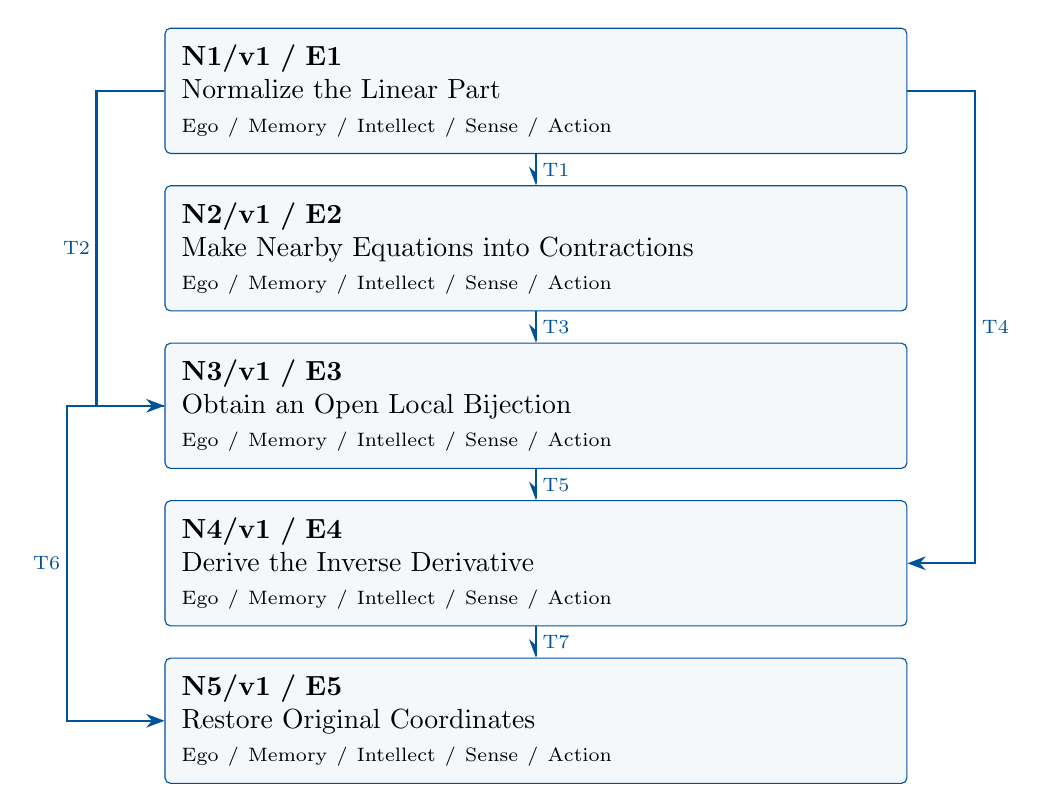
\begin{tikzpicture}[>=Stealth,x=1cm,y=1cm]

\node[mmnode,text width=9cm,minimum height=1.25cm] (N1) at (0,0.0) {\textbf{N1/v1 / E1}\\Normalize the Linear Part\\{\scriptsize Ego / Memory / Intellect / Sense / Action}};

\node[mmnode,text width=9cm,minimum height=1.25cm] (N2) at (0,-2.0) {\textbf{N2/v1 / E2}\\Make Nearby Equations into Contractions\\{\scriptsize Ego / Memory / Intellect / Sense / Action}};

\node[mmnode,text width=9cm,minimum height=1.25cm] (N3) at (0,-4.0) {\textbf{N3/v1 / E3}\\Obtain an Open Local Bijection\\{\scriptsize Ego / Memory / Intellect / Sense / Action}};

\node[mmnode,text width=9cm,minimum height=1.25cm] (N4) at (0,-6.0) {\textbf{N4/v1 / E4}\\Derive the Inverse Derivative\\{\scriptsize Ego / Memory / Intellect / Sense / Action}};

\node[mmnode,text width=9cm,minimum height=1.25cm] (N5) at (0,-8.0) {\textbf{N5/v1 / E5}\\Restore Original Coordinates\\{\scriptsize Ego / Memory / Intellect / Sense / Action}};

\draw[mmproof] (N1.south) -- node[mmnote,right] {T1} (N2.north);

\draw[mmproof] (N1.west) -- (-5.58,0) -- node[mmnote,left] {T2} (-5.58,-4) -- (N3.west);

\draw[mmproof] (N2.south) -- node[mmnote,right] {T3} (N3.north);

\draw[mmproof] (N1.east) -- (5.58,0) -- node[mmnote,right] {T4} (5.58,-6) -- (N4.east);

\draw[mmproof] (N3.south) -- node[mmnote,right] {T5} (N4.north);

\draw[mmproof] (N3.west) -- (-5.96,-4) -- node[mmnote,left] {T6} (-5.96,-8) -- (N5.west);

\draw[mmproof] (N4.south) -- node[mmnote,right] {T7} (N5.north);

\end{tikzpicture}\end{center}

Each box is one mathematical agent containing all five faculties. Blue
arrows carry the versioned exports listed below. The layout gives a
reading order; only drawn arrows assert dependencies. Diagnostic repair
is separate from the proof DAG.

\clearpage\subsection{Versioned evidence-transfer ledger}

\begingroup\small\linespread{1.05}\selectfont

\Needspace{5\baselineskip}\field{T1: N1/E1/v1 to N2}{\(G(z)=L^{-1}(F(a+z)-F(a))\) has \(DG(0)=I\) and \(E=G-I\) is
\(1/2\)-Lipschitz on a closed ball of radius \(\rho\).}

\field{Receiving activity}{N2: Make Nearby Equations into Contractions}

\field{Compatibility}{Use the same mathematical objects and hypotheses as the source export.
Receiving contract: N1/E1; completeness of the closed Euclidean ball.}

\Needspace{5\baselineskip}\field{T2: N1/E1/v1 to N3}{\(G(z)=L^{-1}(F(a+z)-F(a))\) has \(DG(0)=I\) and \(E=G-I\) is
\(1/2\)-Lipschitz on a closed ball of radius \(\rho\).}

\field{Receiving activity}{N3: Obtain an Open Local Bijection}

\field{Compatibility}{Use the same mathematical objects and hypotheses as the source export.
Receiving contract: N1/E1, N2/E2, and the imported Banach contraction
theorem.}

\Needspace{5\baselineskip}\field{T3: N2/E2/v1 to N3}{For \(\|y\|<\rho/2\), \(T_y(z)=y-E(z)\) is a contraction mapping
\(\overline B_\rho\) into itself.}

\field{Receiving activity}{N3: Obtain an Open Local Bijection}

\field{Compatibility}{Use the same mathematical objects and hypotheses as the source export.
Receiving contract: N1/E1, N2/E2, and the imported Banach contraction
theorem.}

\Needspace{5\baselineskip}\field{T4: N1/E1/v1 to N4}{\(G(z)=L^{-1}(F(a+z)-F(a))\) has \(DG(0)=I\) and \(E=G-I\) is
\(1/2\)-Lipschitz on a closed ball of radius \(\rho\).}

\field{Receiving activity}{N4: Derive the Inverse Derivative}

\field{Compatibility}{Use the same mathematical objects and hypotheses as the source export.
Receiving contract: N1/E1 and N3/E3; the Neumann-series inverse bound.}

\Needspace{5\baselineskip}\field{T5: N3/E3/v1 to N4}{\(G:V_0\to B_{\rho/2}\) is a bijection with a \(2\)-Lipschitz inverse
\(H_0\), where \(V_0=B_\rho\cap G^{-1}(B_{\rho/2})\) is open.}

\field{Receiving activity}{N4: Derive the Inverse Derivative}

\field{Compatibility}{Use the same mathematical objects and hypotheses as the source export.
Receiving contract: N1/E1 and N3/E3; the Neumann-series inverse bound.}

\Needspace{5\baselineskip}\field{T6: N3/E3/v1 to N5}{\(G:V_0\to B_{\rho/2}\) is a bijection with a \(2\)-Lipschitz inverse
\(H_0\), where \(V_0=B_\rho\cap G^{-1}(B_{\rho/2})\) is open.}

\field{Receiving activity}{N5: Restore Original Coordinates}

\field{Compatibility}{Use the same mathematical objects and hypotheses as the source export.
Receiving contract: N3/E3 and N4/E4 with the fixed affine coordinate
changes.}

\Needspace{5\baselineskip}\field{T7: N4/E4/v1 to N5}{\(DH_0(y)=DG(H_0(y))^{-1}\) exists and is continuous.}

\field{Receiving activity}{N5: Restore Original Coordinates}

\field{Compatibility}{Use the same mathematical objects and hypotheses as the source export.
Receiving contract: N3/E3 and N4/E4 with the fixed affine coordinate
changes.}

\endgroup

\clearpage\section{Agent roles and five-faculty activities}\begingroup\small\linespread{1.05}\selectfont\setlist{itemsep=1pt,topsep=2pt}

\subsection{N1/v1: Normalize the Linear Part}

\field{Object and role}{Normalize the Linear Part. Establish the following local result:
\(G(z)=L^{-1}(F(a+z)-F(a))\) has \(DG(0)=I\) and \(E=G-I\) is
\(1/2\)-Lipschitz on a closed ball of radius \(\rho\).}

\field{Inputs}{\(F\in C^1(U,\mathbb R^n)\), \(a\in U\), and \(L=DF(a)\) invertible.}

\mmfaculty{E}{Ego}{Own E1/v1: \(G(z)=L^{-1}(F(a+z)-F(a))\) has \(DG(0)=I\) and \(E=G-I\) is
\(1/2\)-Lipschitz on a closed ball of radius \(\rho\).}

\mmfaculty{M}{Memory}{Jacobian and linear inverses}

\mmfaculty{I}{Intellect}{Make derivative identity at zero}

\mmfaculty{S}{Sense}{Require invertible L}

\mmfaculty{A}{Action}{Carry out the numbered deductions and publish E1/v1 together with its
hypotheses and proof location.}

\smallskip\noindent\textbf{Numbered mathematical activities}

\begin{enumerate}[label=N1.\arabic*,leftmargin=3.4em]

\item Translate \(a\) and \(F(a)\) to zero and multiply by \(L^{-1}\).

\item Use continuity of \(DG\) to choose a closed ball inside the transformed
domain with \(\|DG-I\|\le1/2\).

\item Integrate \(DE\) along segments to obtain the Lipschitz estimate.

\end{enumerate}

\field{Export E1/v1}{\(G(z)=L^{-1}(F(a+z)-F(a))\) has \(DG(0)=I\) and \(E=G-I\) is
\(1/2\)-Lipschitz on a closed ball of radius \(\rho\).}

\field{Acceptance gate}{Require invertible L Publish only after checking every displayed
deduction.}

\field{Targeted repair}{If the check fails, revise N1: Require invertible L Recheck dependent
nodes N2, N3, N4, N5.}

\clearpage

\subsection{N2/v1: Make Nearby Equations into Contractions}

\field{Object and role}{Make Nearby Equations into Contractions. Establish the following local
result: For \(\|y\|<\rho/2\), \(T_y(z)=y-E(z)\) is a contraction mapping
\(\overline B_\rho\) into itself.}

\field{Inputs}{N1/E1; completeness of the closed Euclidean ball.}

\mmfaculty{E}{Ego}{Own E2/v1: For \(\|y\|<\rho/2\), \(T_y(z)=y-E(z)\) is a contraction
mapping \(\overline B_\rho\) into itself.}

\mmfaculty{M}{Memory}{Derivative continuity and segment estimates}

\mmfaculty{I}{Intellect}{Recast equation as fixed point}

\mmfaculty{S}{Sense}{Check complete invariant ball}

\mmfaculty{A}{Action}{Carry out the numbered deductions and publish E2/v1 together with its
hypotheses and proof location.}

\smallskip\noindent\textbf{Numbered mathematical activities}

\begin{enumerate}[label=N2.\arabic*,leftmargin=3.4em]

\item Estimate \(\|T_y(z)-T_y(w)\|\le\|z-w\|/2\).

\item Use \(E(0)=0\) to prove \(\|T_y(z)\|\le\|y\|+\|z\|/2<\rho\).

\item Check both the uniform contraction constant and the self-map condition
before applying Banach.

\end{enumerate}

\field{Export E2/v1}{For \(\|y\|<\rho/2\), \(T_y(z)=y-E(z)\) is a contraction mapping
\(\overline B_\rho\) into itself.}

\field{Acceptance gate}{Check complete invariant ball Publish only after checking every
displayed deduction.}

\field{Targeted repair}{If the check fails, revise N2: Check complete invariant ball Recheck
dependent nodes N3, N4, N5.}

\clearpage

\subsection{N3/v1: Obtain an Open Local Bijection}

\field{Object and role}{Obtain an Open Local Bijection. Establish the following local result:
\(G:V_0\to B_{\rho/2}\) is a bijection with a \(2\)-Lipschitz inverse
\(H_0\), where \(V_0=B_\rho\cap G^{-1}(B_{\rho/2})\) is open.}

\field{Inputs}{N1/E1, N2/E2, and the imported Banach contraction theorem.}

\mmfaculty{E}{Ego}{Own E3/v1: \(G:V_0\to B_{\rho/2}\) is a bijection with a \(2\)-Lipschitz
inverse \(H_0\), where \(V_0=B_\rho\cap G^{-1}(B_{\rho/2})\) is open.}

\mmfaculty{M}{Memory}{Banach existence and uniqueness}

\mmfaculty{I}{Intellect}{Separate onto and one-to-one}

\mmfaculty{S}{Sense}{Keep solutions inside open neighborhood}

\mmfaculty{A}{Action}{Carry out the numbered deductions and publish E3/v1 together with its
hypotheses and proof location.}

\smallskip\noindent\textbf{Numbered mathematical activities}

\begin{enumerate}[label=N3.\arabic*,leftmargin=3.4em]

\item For each target, solve \(z=T_y(z)\) uniquely on the closed ball.

\item Use the strict self-map bound to place the solution inside the open
ball.

\item Prove \(\|G(z)-G(w)\|\ge\|z-w\|/2\) and deduce inverse continuity and
injectivity.

\end{enumerate}

\field{Export E3/v1}{\(G:V_0\to B_{\rho/2}\) is a bijection with a \(2\)-Lipschitz inverse
\(H_0\), where \(V_0=B_\rho\cap G^{-1}(B_{\rho/2})\) is open.}

\field{Acceptance gate}{Keep solutions inside open neighborhood Publish only after checking
every displayed deduction.}

\field{Targeted repair}{If the check fails, revise N3: Keep solutions inside open neighborhood
Recheck dependent nodes N4, N5.}

\clearpage

\subsection{N4/v1: Derive the Inverse Derivative}

\field{Object and role}{Derive the Inverse Derivative. Establish the following local result:
\(DH_0(y)=DG(H_0(y))^{-1}\) exists and is continuous.}

\field{Inputs}{N1/E1 and N3/E3; the Neumann-series inverse bound.}

\mmfaculty{E}{Ego}{Own E4/v1: \(DH_0(y)=DG(H_0(y))^{-1}\) exists and is continuous.}

\mmfaculty{M}{Memory}{First-order remainder and matrix bounds}

\mmfaculty{I}{Intellect}{Solve increment relation}

\mmfaculty{S}{Sense}{Do not assume differentiability of inverse}

\mmfaculty{A}{Action}{Carry out the numbered deductions and publish E4/v1 together with its
hypotheses and proof location.}

\smallskip\noindent\textbf{Numbered mathematical activities}

\begin{enumerate}[label=N4.\arabic*,leftmargin=3.4em]

\item From \(\|DG-I\|\le1/2\) obtain invertibility and \(\|DG^{-1}\|\le2\).

\item Put \(h=H_0(y+k)-H_0(y)\); the Lipschitz bound gives \(\|h\|\le2\|k\|\).

\item Solve \(k=DG(H_0(y))h+o(\|h\|)\) for \(h\) and then use continuity of
matrix inversion.

\end{enumerate}

\field{Export E4/v1}{\(DH_0(y)=DG(H_0(y))^{-1}\) exists and is continuous.}

\field{Acceptance gate}{Do not assume differentiability of inverse Publish only after checking
every displayed deduction.}

\field{Targeted repair}{If the check fails, revise N4: Do not assume differentiability of
inverse Recheck dependent nodes N5.}

\clearpage

\subsection{N5/v1: Restore Original Coordinates}

\field{Object and role}{Restore Original Coordinates. Establish the following local result:
\(F:V\to W\) is a \(C^1\) diffeomorphism and
\(D(F^{-1})(Y)=DF(F^{-1}(Y))^{-1}\).}

\field{Inputs}{N3/E3 and N4/E4 with the fixed affine coordinate changes.}

\mmfaculty{E}{Ego}{Own E5/v1: \(F:V\to W\) is a \(C^1\) diffeomorphism and
\(D(F^{-1})(Y)=DF(F^{-1}(Y))^{-1}\).}

\mmfaculty{M}{Memory}{All local certificates}

\mmfaculty{I}{Intellect}{Transport inverse and derivative}

\mmfaculty{S}{Sense}{Restore original coordinates}

\mmfaculty{A}{Action}{Carry out the numbered deductions and publish E5/v1 together with its
hypotheses and proof location.}

\smallskip\noindent\textbf{Numbered mathematical activities}

\begin{enumerate}[label=N5.\arabic*,leftmargin=3.4em]

\item Set \(V=a+V_0\) and \(W=F(a)+L B_{\rho/2}\).

\item Define \(H(Y)=a+H_0(L^{-1}(Y-F(a)))\) and check both inverse identities.

\item Apply the chain rule to transport the derivative formula to the original
coordinates.

\end{enumerate}

\field{Export E5/v1}{\(F:V\to W\) is a \(C^1\) diffeomorphism and
\(D(F^{-1})(Y)=DF(F^{-1}(Y))^{-1}\).}

\field{Acceptance gate}{Restore original coordinates Publish only after checking every displayed
deduction.}

\field{Targeted repair}{If the check fails, revise N5: Restore original coordinates Withhold
this terminal result until its gate passes.}

\endgroup\clearpage\section{Continuous mathematical proof}\label{sec:proof}

\subsection{N1 --- Normalize the Linear
Part}\label{n1-normalize-the-linear-part}

Set

\[G(z)=L^{-1}\big(F(a+z)-F(a)\big).\]

Then \(G(0)=0\) and \(DG(0)=I\). Its domain is an open neighborhood of
zero. By continuity of DG choose \(\rho >0\) such that the closed
Euclidean ball \(\overline B_\rho\) lies in that domain and

\[\|DG(z)-I\|\le\tfrac12\quad(z\in\overline B_\rho).\]

Write \(E(z)=G(z)-z\). For x,z in this ball the connecting segment
remains inside it, and integration of DE along that segment gives

\[\|E(x)-E(z)\|\le\tfrac12\|x-z\|.\]

In particular \(E(0)=0\) and \(\Vert E(z)\Vert \le \Vert z\Vert /2\).

\subsection{N2 --- Make Nearby Equations into
Contractions}\label{n2-make-nearby-equations-into-contractions}

For a normalized target y with \(\Vert y\Vert <\rho /2\), define

\[T_y(z)=y-E(z)=z-G(z)+y.\]

Its fixed points are exactly the solutions \(G(z)=y\). The previous
estimate gives contraction factor 1/2. Also

\[\|T_y(z)\|\le\|y\|+\tfrac12\rho<\rho\]

for z in the closed ball. Thus \(T_y\) maps a complete ball into itself.
Both conditions are required to import Banach's theorem.

\subsection{N3 --- Obtain an Open Local
Bijection}\label{n3-obtain-an-open-local-bijection}

Banach gives exactly one solution in the closed ball, and the strict
self-map bound places it in the open ball. Separately, for x,z in the
closed ball,

\[\|G(x)-G(z)\|\ge\|x-z\|-\|E(x)-E(z)\|\ge\tfrac12\|x-z\|.\]

Hence G is injective on the ball. Put

\[W_0=B_{\rho/2},\qquad V_0=B_\rho\cap G^{-1}(W_0).\]

The set \(V_0\) is open, contains zero, and G maps it bijectively onto
\(W_0\). Let \(H_0\) be its inverse. Applying the lower bound to
\(H_0(y),H_0(y\)') gives

\[\|H_0(y)-H_0(y')\|\le2\|y-y'\|.\]

So the inverse is Lipschitz and in particular continuous. This does not
yet establish its differentiability.

\subsection{N4 --- Derive the Inverse
Derivative}\label{n4-derive-the-inverse-derivative}

Every \(DG(x)\) on the ball is invertible: \(\|DG(x)-I\|\le1/2\) permits
the convergent matrix geometric series for its inverse, with inverse
norm at most 2.

Fix y in \(W_0\) and \(x=H_0(y)\). For small k with y+k in \(W_0\), set
\(h=H_0(y+k)-H_0(y)\). The Lipschitz bound gives
\(\Vert h\Vert \le 2\Vert k\Vert\). Differentiability of G at x gives

\[k=G(x+h)-G(x)=DG(x)h+r(h),\qquad\|r(h)\|=o(\|h\|).\]

Therefore

\[h=DG(x)^{-1}k-DG(x)^{-1}r(h)=DG(x)^{-1}k+o(\|k\|).\]

The remainder conversion is justified by
\(\Vert h\Vert \le 2\Vert k\Vert\) and the bounded inverse matrix. Thus
\(DH_0(y)=DG(H_0(y))^{-1}\). This derivative is continuous because
\(H_0\) and DG are continuous and matrix inversion is continuous on
invertible matrices. Hence \(H_0\) is \(C^{1}\).

\subsection{N5 --- Restore Original
Coordinates}\label{n5-restore-original-coordinates}

Choose \(V=a+V_0\) and \(W=F(a)+L\) \(W_0\). These are open
neighborhoods. Their inverse is

\[H(Y)=a+H_0\big(L^{-1}(Y-F(a))\big).\]

The chain rule gives \(DH(Y)=DF(H(Y))^{-1}\). All four obligations are
now proved, so the original-coordinate theorem follows. \(\square\)

\hfill$\square$

\section{Worked orchestration}

Let \(F(x,y)=(x+y^2,y+x^2)\) at \(a=(0,0)\). Its derivative at zero is
I. On the closed Euclidean ball of radius \(\rho =1/4\),

\[DF-I=\begin{pmatrix}0&2y\\2x&0\end{pmatrix},\qquad\|DF-I\|=2\max(|x|,|y|)\le\tfrac12.\]

Thus every target of norm less than 1/8 has exactly one preimage in the
chosen local neighborhood. The fixed-point update is

\[(x,y)\longmapsto(u-y^2,v-x^2).\]

For target \((u,v)=(1/20,1/20)\), symmetry gives \(x=y=s\), where

\[s+s^2=\tfrac1{20},\qquad s=\frac{\sqrt{6/5}-1}{2}\approx0.0477225575.\]

The negative quadratic root is outside the local ball and does not
contradict local uniqueness. At this preimage,

\[DH=\frac1{1-4s^2}\begin{pmatrix}1&-2s\\-2s&1\end{pmatrix}.\]

The Banach module also supplies an error bound for the numerical
iteration, using \(q=1/2\).

\subsection{Boundary and hypothesis audit}

At \(F(x)=x^{3}\) near zero, the inverse exists as a continuous map but
fails the claimed differentiability; \(DF(0)\) is not invertible. Polar
coordinates are locally invertible away from \(r=0\) but remain globally
periodic in angle. These distinguish failure of a sufficient hypothesis
from impossibility of every inverse.

Export the normalized contraction construction, local inverse, Lipschitz
bound, and \(C^{1}\) derivative formula. The example explicitly
demonstrates a theorem module imported from another subject's graph.

\section{Illustrative failure and repair}

The following is an authored diagnostic scenario. Changed assumptions
define a new contract; they do not retroactively prove the original
statement.

\subsection{Failure and correction}
\begin{itemize}
\item
  \textbf{Interaction}

  N1 \(\to\) N2

  \textbf{Certificate}

  Normalized map and uniform derivative bound on the closed ball
\item
  \textbf{Interaction}

  N2 \(\to\) N3

  \textbf{Certificate}

  Complete self-map, contraction 1/2, target-radius restriction
\item
  \textbf{Interaction}

  Banach \(\to\) N3

  \textbf{Certificate}

  Unique fixed point for each admissible target
\item
  \textbf{Interaction}

  N3 \(\to\) N4

  \textbf{Certificate}

  Local inverse and Lipschitz factor 2
\item
  \textbf{Interaction}

  N4 \(\to\) N5

  \textbf{Certificate}

  \(C^{1}\) inverse with proved derivative formula
\item
  \textbf{Interaction}

  N5 \(\to\) caller

  \textbf{Certificate}

  Open neighborhoods in original coordinates
\end{itemize}

A failed branch selects a large target but reuses the small-ball
certificate. For the example, a target with norm 1 is not covered by the
radius-1/8 guarantee.

\begin{itemize}
\item
  \textbf{Node:} N2
\item
  \textbf{State:} STALLED
\item
  \textbf{Failing faculty:} Sense
\item
  \textbf{Failed hypothesis:} target norm \(<\) rho/2
\item
  \textbf{Observed:} target norm 1, \(\rho =1/4\)
\item
  \textbf{Repair target:} target/domain contract
\item
  \textbf{Blocked export:} small-ball existence certificate
\end{itemize}

Memory retrieves the radius relation. Sense retains the target mismatch.
Intellect either restricts the target or develops a new valid
neighborhood. Action rechecks the self-map estimate. Ego publishes only
the result supported by that estimate; failure of this certificate alone
is not proof that a large-target solution does not exist.

\subsection{Hypothesis boundary}
At \(F(x)=x^{3}\) near zero, the inverse exists as a continuous map but
fails the claimed differentiability; \(DF(0)\) is not invertible. Polar
coordinates are locally invertible away from \(r=0\) but remain globally
periodic in angle. These distinguish failure of a sufficient hypothesis
from impossibility of every inverse.

Export the normalized contraction construction, local inverse, Lipschitz
bound, and \(C^{1}\) derivative formula. The example explicitly
demonstrates a theorem module imported from another subject's graph.

\subsection{Version and recheck}
Treat any changed assumption as a new contract. Recheck the revised
export and all of its descendants. A backward diagnostic never
establishes an earlier theorem. This is an authored teaching trace, not
an execution log.

\par\medskip\begingroup\small\linespread{1.0}\selectfont\noindent\textbf{Provenance.} This authored proof is complete relative to its declared imports. Reuse
each export with its assumptions, proof, and version. The original
Markdown remains available for comparison.
\par\endgroup

\par\smallskip\begingroup\small\linespread{1.0}\selectfont\noindent\textbf{Further reading.} \href{https://www2.math.upenn.edu/~gressman/analysis/12-inversefuncthm.html}{University
of Pennsylvania: contraction-based proof of the inverse function
theorem}.\par\endgroup

\end{document}
